\documentclass[10pt, xcolor=pdflatex, dvipsnames, table]{beamer}
%------------------  xcolor,         jmena barev, colortbl/rowcolors

%\usepackage{czech}    % pokud chceme ceske labely
\usepackage{graphicx}  % obrazky
\usepackage{newcent}   % Century Gothic FONT

\usetheme[tocnumbers]{FIT} 
\usepackage{ucs}
\usepackage[utf8x]{inputenc}
\usepackage[czech]{babel}
\usepackage{palatino}
\usepackage{graphicx}
\usepackage{textcomp}
\usepackage{algorithm}
\usepackage{algorithmicx}
\usepackage{algpseudocode}
\usepackage{wrapfig}
\usepackage{siunitx}

\title{Fourierovská optika -- úpravy obrazu.}
\author{Jan Wozniak}
\institute[FIT VUT]{Vysoké učení technické v~Brně\\
Fakulta informační technologií}
\date{\today}

\begin{document}

\begin{frame}[plain]
\titlepage
\end{frame}

\begin{frame}
\frametitle{Úvod}
\textbf{Fraunhoferova difrakce}
\begin{itemize}
\item převod do frekvenční oblasti
\item inertibilní
\end{itemize}

\vspace{1em}

\textbf{Rovina s Fraunhoferovou difrakcí} 
\begin{itemize}
\item bez optické soustavy těžce sledovatelná
\end{itemize}

\vspace{1em}

Matematická alternativa -- \textit{Fourierova transformace}

\vspace{1em}

\begin{center}
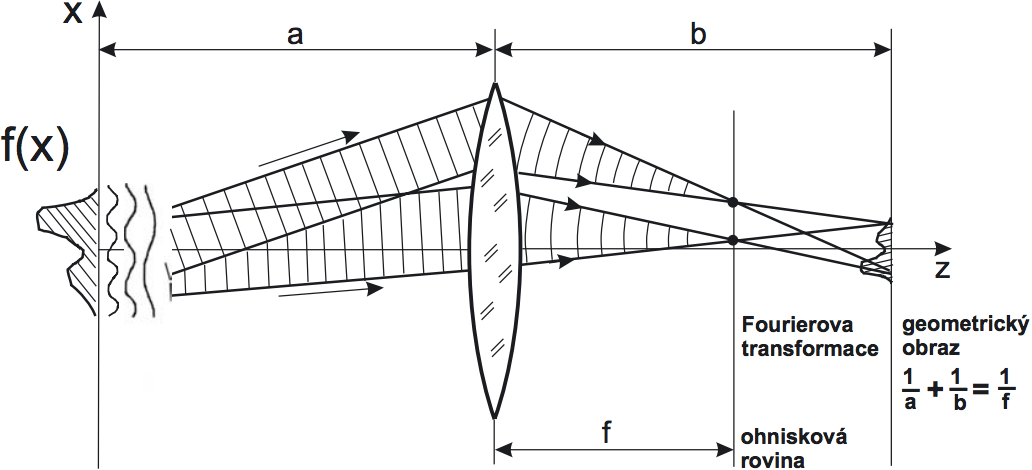
\includegraphics[width=8cm]{images/ft-cocka.png}
\end{center}
\end{frame}

\begin{frame}
\frametitle{Fourierova transformace}

\textbf{Princip} 
\begin{itemize}
  \item převod z prostorové do frekvenční oblasti
  \item signál lze vyjádřit jako suma komplexních kosínusovek
  \item počítá se na základě intenzity pixelu
  \item spektrum souměrné podle diagonál
\end{itemize} 

\begin{center}
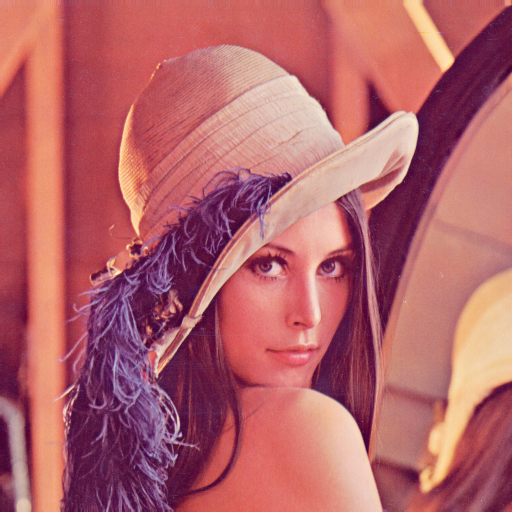
\includegraphics[width=4cm]{images/lena.png}
\hspace{1em}
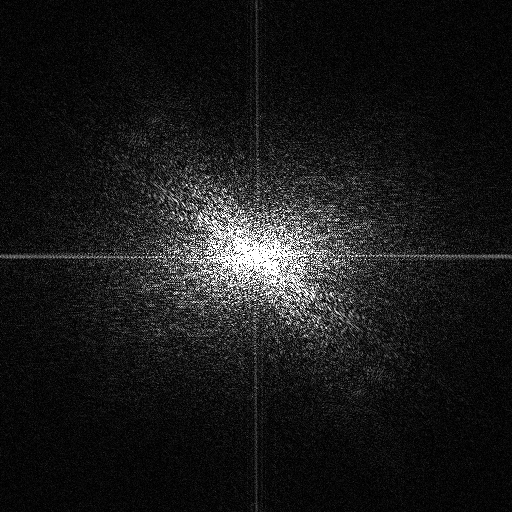
\includegraphics[width=4cm]{images/lena_spec.png}
\end{center}
\end{frame}






\begin{frame}
\frametitle{Filtrace ve frekvenční oblasti}
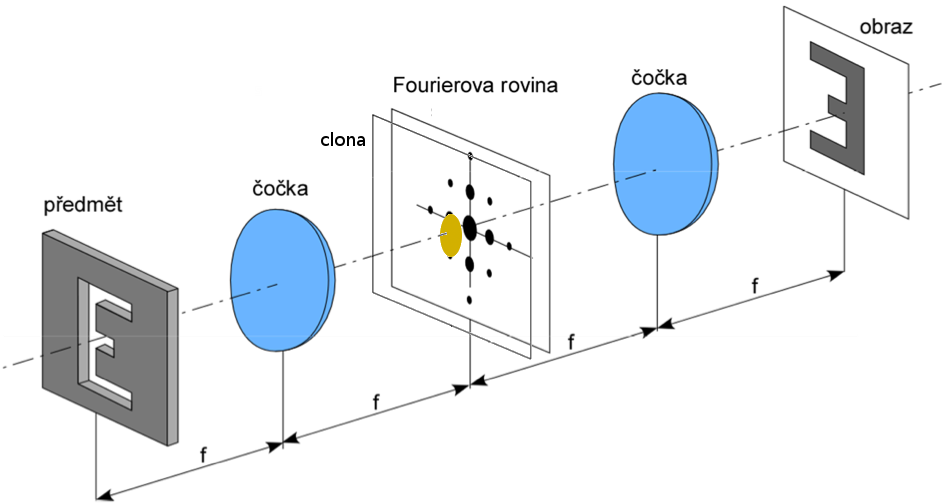
\includegraphics[width=11cm]{images/dft.png}
\end{frame}





\begin{frame}
\frametitle{Asymptotická časová složitost}
\textbf{Filtrace obrazu..}

\vspace{1em}

\textbf{..ve frekvenční oblasti}
\begin{itemize}
\item $F[k,l] = \sum_{m=0}^{N}{\sum_{n=0}^{N}{f[m,n]e^{(-i)\frac{2\pi km}{N}}\cdot e^{(-i)\frac{2\pi ln}{N}}}}$
\item Fast Fourier Transform
\item $\mathcal{O}(N^2 \cdot \log_{2}{N})$ 
\end{itemize}

\vspace{1em}

\textbf{..v prostorové oblasti}
\begin{itemize}
\item $g[m,n] = \sum_{k=0}^{N}{\sum_{l=0}^{N}{f[k,l]\cdot h[m-k, n-l]}}$
\item $\mathcal{O}(N^2 \cdot M^2)$ 
\end{itemize}

\end{frame}





\begin{frame}
\frametitle{Využití}
\textbf{Fyzikální využití}
\begin{itemize}
\item analýza snímků elektronového mikroskopu
\item kontrola tloušťky vláken
\item korekce zobrazování v optických soustavách
\end{itemize}

\vspace{1em}

\textbf{Transformace do frekvenční oblasti}
\begin{itemize}
\item Gáborův filter -- krátkodobá FT + Gaussovo okno 
\item kompresní formáty -- JPEG, PNG
\end{itemize}
\end{frame}


\frame[plain]{\bluepage{Děkuji za pozornost}}
\end{document}
